\documentclass{cmspaper}
\usepackage{color}
\usepackage{graphicx}
\usepackage{wrapfig}
\usepackage{slashbox}
\usepackage{epstopdf}  %added for MAC compiler
\usepackage{pdfpages}
\usepackage{lineno}
\usepackage{verbatim}
\usepackage{url}
\RequirePackage{lineno} 
%\RequirePackage{lineno} 

\usepackage{wrapfig}

%Note to authors: these definitions are suggested to be used for consistency
\newcommand{\pt}{$p_T$ }
\newcommand{\GeVc}{GeV/c}
\newcommand{\mll}{\ensuremath{M_{\ell\ell}}}
\newcommand{\z}{$Z$ }
\newcommand{\zjets}{$\rm{Z}+\rm{jets}$ }
\newcommand{\gjets}{$\gamma+\rm{jets}$ }
\newcommand{\Z}{$Z$ } %redundancy can be good
\newcommand{\ttbar}{\ensuremath{t\bar{t}}}
\newcommand{\emu }{\ensuremath{e\mu}}
\newcommand{\ee  }{\ensuremath{ee}}
\newcommand{\eepm}{\ensuremath{e^+ e^-}}
\newcommand{\mm  }{\ensuremath{\mu\mu}}
\newcommand{\mmpm}{\ensuremath{\mu^+ \mu^-}}
\newcommand{\empm}{\ensuremath{e^\pm \mu^\mp}}
\newcommand{\ase}[2]{\ensuremath{_{~- #1}^{~+ #2}}}
\newcommand{\MET}{\ensuremath{\rm{E_{T}^{miss}}}}
\newcommand{\met}{\mbox{$\raisebox{.3ex}{$\not$}E_T$\hspace*{0.5ex}}} 
\newcommand{\effr}{$R_{e\mu}$} %used to be \epsilon
\newcommand{\effrm}{$R_{\mu e}$} %used to be \epsilon
\newcommand{\sta}{$\sigma\times A$} %notation is such that A includes BR
\newcommand{\statistics}{CL$_\mathrm{S}$}
\newcommand{\njets}{$N_{\rm{jets}}$}

%The lumi so that if it changes it's easier to update
\newcommand{\lumi}{9.2~fb$^{-1}$}

%loose(tight) signal region met cut
\newcommand{\signalmetl}{100}
\newcommand{\signalmett}{200}
\newcommand{\signalmetvt}{300}

\newcommand{\resulttitle}
%{                       &   MET $>30$  GeV    &   MET $>60$  GeV    &   MET $>100$ GeV    &   MET $>200$ GeV \\}
%{                       &   MET $>30$  GeV    &   MET $>60$  GeV    &   MET $>100$ GeV    &   MET $>200$ GeV  &  MET $>300$ GeV  \\}
%move 300 to 150
{                       &   MET $>30$  GeV    &   MET $>60$  GeV    &   MET $>100$ GeV    &   MET $>150$ GeV  &  MET $>200$ GeV  \\}

\newcommand{\wjets}{$\rm{W}+{\rm jets}$}
\newcommand{\zzmet}{$\rm{ZZ}+\MET$}
\newcommand{\wzmet}{$\rm{WZ}+\MET$}
\newcommand{\wzzmet}{$\rm{WZ/ZZ}+\MET$}
\newcommand{\Ht}{$H_{T}$}
\newcommand{\cls}  {\ensuremath{\mathrm{CL_S}}}


\begin{document}


%\begin{comment}

\begin{titlepage}

  %\internalnote{2011/000}
  \cmsnote{2011/XXX}

  \date{\today}
 
  \title{\MET\ Templates Results and Additional Cross-checks for the Opposite-sign Same-flavor (``Edge'') Dilepton Analysis}

  %No Victor this time (sorry, Victor)
  \begin{Authlist}

D.~Barge, A.~George, C.~Campagnari, F.~Golf, J.~Gran, D.~Kovalskyi, V.~Krutelyov
\Instfoot{ucsb}{University of California, Santa Barbara, USA}

G.~Cerati, D.~Evans, R.~Kelley, I.~MacNeill, S.~Padhi, Y.~Tu, F.~W\"urthwein, V.~Welke, A.~Yagil, J.~Yoo
\Instfoot{ucsd}{University of California, San Diego, USA}

L.~Bauerdick, K.~Burkett, I.~Fisk, Y.~Gao, O.~Gutsche, B.~Hooberman, S.~Jindariani, J.~Linacre, V.~Martinez Outschoorn
\Instfoot{fnal}{Fermi National Accelerator Laboratory, Batavia, Illinois, USA}

  \end{Authlist}

  \begin{abstract}

    The Aachen and ETH groups have reported an excess of events with low mass, opposite-sign same-flavor lepton pairs,
    commonly referred to as the ``edge analysis.''
    In this note, we use the \MET\ templates technique to estimate the Z background in the Z mass region for the two
    signal regions used in this analysis. This prediction is extrapolated to low mass to estimate the $\gamma^*/Z$
    contribution. Additional cross-checks are also presented.

  \end{abstract}

\end{titlepage}

%\end{comment}

\setcounter{page}{2}%JPP

\newpage
\tableofcontents

\newpage
\linenumbers
\section{Changes w.r.t. previous AN Version}
\label{sec:changes}

\begin{itemize}

\item v6: Updated to full 2012 sample corresponding to 19.3 fb$^{-1}$.
\item v5: {\bf This is the version corresponding to the HCP results}. Added interpretation for the GMSB model (Sec.~\ref{sec:interpretation}). Added data vs. MC kinematic distributions for the sample with 3 leptons and at least 2 jets, where we observe an excess of data with respect to the MC prediction (App.~\ref{app:WZ}).
\item v4: Un-blinded the results of the inclusive and targeted analysis, and added an interpretation in the \wzmet\ model. Moved the material for the edge analysis to a separate AN (2012/359).
\item v3: Added results for the low-\MET\ and high-\MET\ signal regions used for the edge analysis, for the first 5.1 fb$^{-1}$ 2012A+B data.
\item v2: Updated to 9.2 fb$^{-1}$ of 53X data and MC (v1 used 5.1 fb$^{-1}$ 52X data and MC).

\end{itemize}

\section{Introduction}
\label{sec:intro}

In this note we describe a search for new physics in the 2011 
opposite sign isolated dilepton sample ($ee$, $e\mu$, and $\mu\mu$).  
The main source of 
isolated dileptons at CMS is Drell Yan and $t\bar{t}$.
Here we concentrate on dileptons with invariant mass inconsistent
with $Z \to ee$ and $Z \to \mu\mu$.  Thus $t\bar{t}$ is the most
important background.  A separate search for new physics in the $Z$ 
sample is described in a separate note\cite{ref:Ztemplates}.
This is an update of an analysis performed on 2010 data~\cite{ref:osnote,ref:ospaper}. 

The search strategy is the following

\begin{itemize}

\item We start out with a pre-selection which is as close as 
possible to the published (or soon to be published) $t\bar{t}$
dilepton analysis\cite{ref:top} (same lepton ID, same jet definitions,
etc.).  We do make a couple of substantive modifications:

\begin{enumerate}
\item The top analysis requires two leptons of $P_T > 20$ GeV.  
 In this
analysis we lower the requirement on the second lepton to $P_T > 10$ 
GeV.  This is motivated by our desire to maintain sensitivity to possible
SUSY signals with relatively low $P_T$ leptons generated in the 
cascade decays of heavy objects.
\item The top analysis requires at least two jets of $P_T > 30$
GeV with \met $>30$ GeV ($ee$ and $e\mu$) or \met $>20$ GeV ($e \mu$).
We tighten the \met cut to 50 GeV and we 
also require that the scalar sum of the $P_T$ of all jets with $P_T > 30$
GeV be $> 100$ GeV.  These requirements considerably
reduce backgrounds to the $t\bar{t}$ sample, {\em e.g.}, backgrounds
from Drell Yan and $W+$jets.
\end{enumerate}

\item The pre-selection consists mostly of $t\bar{t}$ events.  We perform 
data $-$ Monte Carlo comparisons of kinematical distributions.  Assuming
reasonable agreeement for the bulk of $t\bar{t}$ we move on to a 
search for new physics in the tail of the $t\bar{t}$.

\item Our prejudice is that new physics would manifest itself in an
excess of events with high \met and significant hadronic activity.
We define an a-priori search region by tightening the \met and 
hadronic activity requirements such that we expect of order 1\% 
of $t\bar{t}$ events to pass the selection (as predicted by Monte Carlo).

\item We perform a counting experiment in the signal region.  We compare
observed yields with expectations from Monte Carlo and with two independent
data driven techniques (see Section~\ref{sec:abcd} and~\ref{sec:victory}).

\end{itemize}




\input{sync.tex}
\clearpage
\section{Results of the \MET\ Templates Analysis}
\label{sec:templates}

In this section, we use the \MET\ templates technique to derive predictions for the background in the on-Z region for the 
four signal regions used for the edge analysis. The background estimation methodology used in the \MET\ templates analysis
is described in AN-2012/254; this AN presents only details which differ from that reference. 
We then use the predicted Z background to derive an estimate of the low-mass $\gamma^*$/Z contribution,
using an extrapolation technique commonly referred to as the ``$R_{out/in}$'' technique~\cite{ref:routin}.

\subsection{Background Estimation Methodology}
\label{sec:templates_bkg}

The strategy is to select Z$\to\ell\ell$ candidates ($81<m_{\ell\ell}<101$ GeV) with jet requirements corresponding to the
low-\MET\ and high-\MET\ signal regions, and compare the observed \MET\ distribution to the sum of the predictions from the 
four background categories:

\begin{itemize}
\item \zjets\ background: the \MET\ in \zjets\ events is modeled using a data control sample of \gjets\ events. These events are reweighted
to account for different jet kinematics in \zjets\ vs. \gjets\ events using the ``\MET\ templates'' technique.
\item Flavor-symmetric (FS) background: this background category is dominated by \ttbar, and consists of processes with equal rates for same-flavor (ee and $\mu\mu$)
vs. opposite-flavor (e$\mu$) events. The FS background is predicted from the e$\mu$ data sample. The on-Z dilepton mass requirement is not applied to the e$\mu$ sample,
and the predictions are scaled by $K$, the MC efficiency for e$\mu$ background events to satisfy the on-Z dilepton mass requirement.
\item WZ/ZZ background: this background is predicted from MC, after validation in 3-lepton (WZ) and 4-lepton (ZZ) data control samples. The contributions from WZ and ZZ to the FS background estimate are negligible.
\item Rare background: this background consists of processes with Z bosons ($t\bar{t}\rm{Z}$ and ZZZ, ZZW, ZWW) that have small cross sections, and is estimated from MC.
\end{itemize}

In order to adapt the \MET\ templates method to predict the Z background in these regions, we make minor modifications
to the procedure used in AN-2012/254. Specifically, we re-calculate
the FS scaling factor $K$ and change the binning used for the \MET\ templates.
The details of the extraction of $K$ are presented in App.~\ref{app:k}; to summarize, we use $K=0.14\pm0.02$ for 
signal regions with inclusive leptons and $K=0.15\pm0.02$ for signal regions with central leptons.
%The FS background is estimated using e$\mu$ events in data.
%To improve the precision of this background estimate, the dilepton mass requirement is not applied, and we apply a scaling
%factor $K$, which is the efficiency for e$\mu$ events to fall in the Z mass window,  extracted from MC.
%The systematic uncertainty on $K$ is assessed by comparing this quantity in data vs. MC.
%The values of $K$ for various \MET\ intervals for the high-\MET\ region (using \pt\ $>$ (20,10) GeV leptons and at least 2 jets) 
%are shown in Fig.~\ref{fig:K_incl_highmet}. 
%Based on this plot we choose $K=0.13\pm0.02$ for \MET\ signal regions up to 200 GeV; for \MET\ 200-300 GeV and \MET\ $>$ 300 GeV
%we inflate the uncertainty to $K=0.13\pm0.04$ and $K=0.13\pm0.05$, respectively, due to the limited statistical precision.
%The values of $K$ for the low-\MET\ region (using \pt\ $>$ (20,20) GeV leptons and at least 3 jets) are shown in 
%Fig.~\ref{fig:K_incl_lowmet}. 
%Based on this plot we choose $K=0.14\pm0.02$ for \MET\ signal regions up to 200 GeV; for \MET\ 200-300 GeV and \MET\ $>$ 300 GeV
%we inflate the uncertainty to $K=0.14\pm0.03$ and $K=0.14\pm0.07$, respectively.
In addition, we change the jet \pt\ threshold for the \MET\ templates jet multiplicity binning from 30 to 40 GeV, and change the $H_T$ bins to
(0,80,100,150,200,250,300,5000) GeV.

\subsection{Results in Z Mass Window}

The results of the for the signal regions with inclusive leptons are displayed in Fig.~\ref{fig:results_inclusive} and summarized in Table~\ref{tab:results_inclusive}.
The results of the for the signal regions with central leptons are displayed in Fig.~\ref{fig:results_central} and summarized in Table~\ref{tab:results_central}.
For all four signal regions, the observed \MET\ distributions agree with the expected \MET\ distributions for the sum of the backgrounds.
The observed yields for the \MET\ $>$ 100 GeV (low-\MET) and \MET\ $>$ 150 GeV (high-\MET) requirements are consistent with the
expected background yields within $\pm1\sigma$. No evidence of a signal-like excess is observed in any region.

%separately for the Run2012A+B data (5.1 fb$^{-1}$) and Run2012C data (4.1 fb$^{-1}$).
%In the Run2012A+B data, we observed a 1.6$\sigma$ excess for \MET\ $>$ 100 GeV, corresponding to the low \MET\ signal region.
%However, this excess does not persist in Run2012C data, where we observe good agreement between the data and the predicted background.
%In the combined Run2012A+B+C data (Fig.~\ref{fig:results_fulledge} and Table~\ref{tab:results_edgefull}) we observe reasonable
%agreement over the full \MET\ range. In the \MET\ $>$ 100 GeV region we observe 288 events with a predicted background of $251\pm33$,
%representing an excess of 1.0$\sigma$.

%The results of the high \MET\ signal region are displayed in Fig.~\ref{fig:results_highmet} and summarized in 
%Table~\ref{tab:results_highmet},
%separately for the Run2012A+B data (5.1 fb$^{-1}$) and Run2012C data (4.1 fb$^{-1}$).
%In both periods we observe good agreement between the data and predicted background over the full \MET\ range.
%In the combined Run2012A+B+C data (Fig.~\ref{fig:results_fulledge} and Table~\ref{tab:results_edgefull}) we observe reasonable
%agreement over the full \MET\ range. 
%In the \MET\ $>$ 150 GeV region corresponding to the high \MET\ signal region in the full sample, we observe 167 events with a predicted
%background of $177\pm25$ events, representing a deficit of -0.4$\sigma$.

\clearpage

\begin{figure}[!h]
\begin{center}
\begin{tabular}{cc}
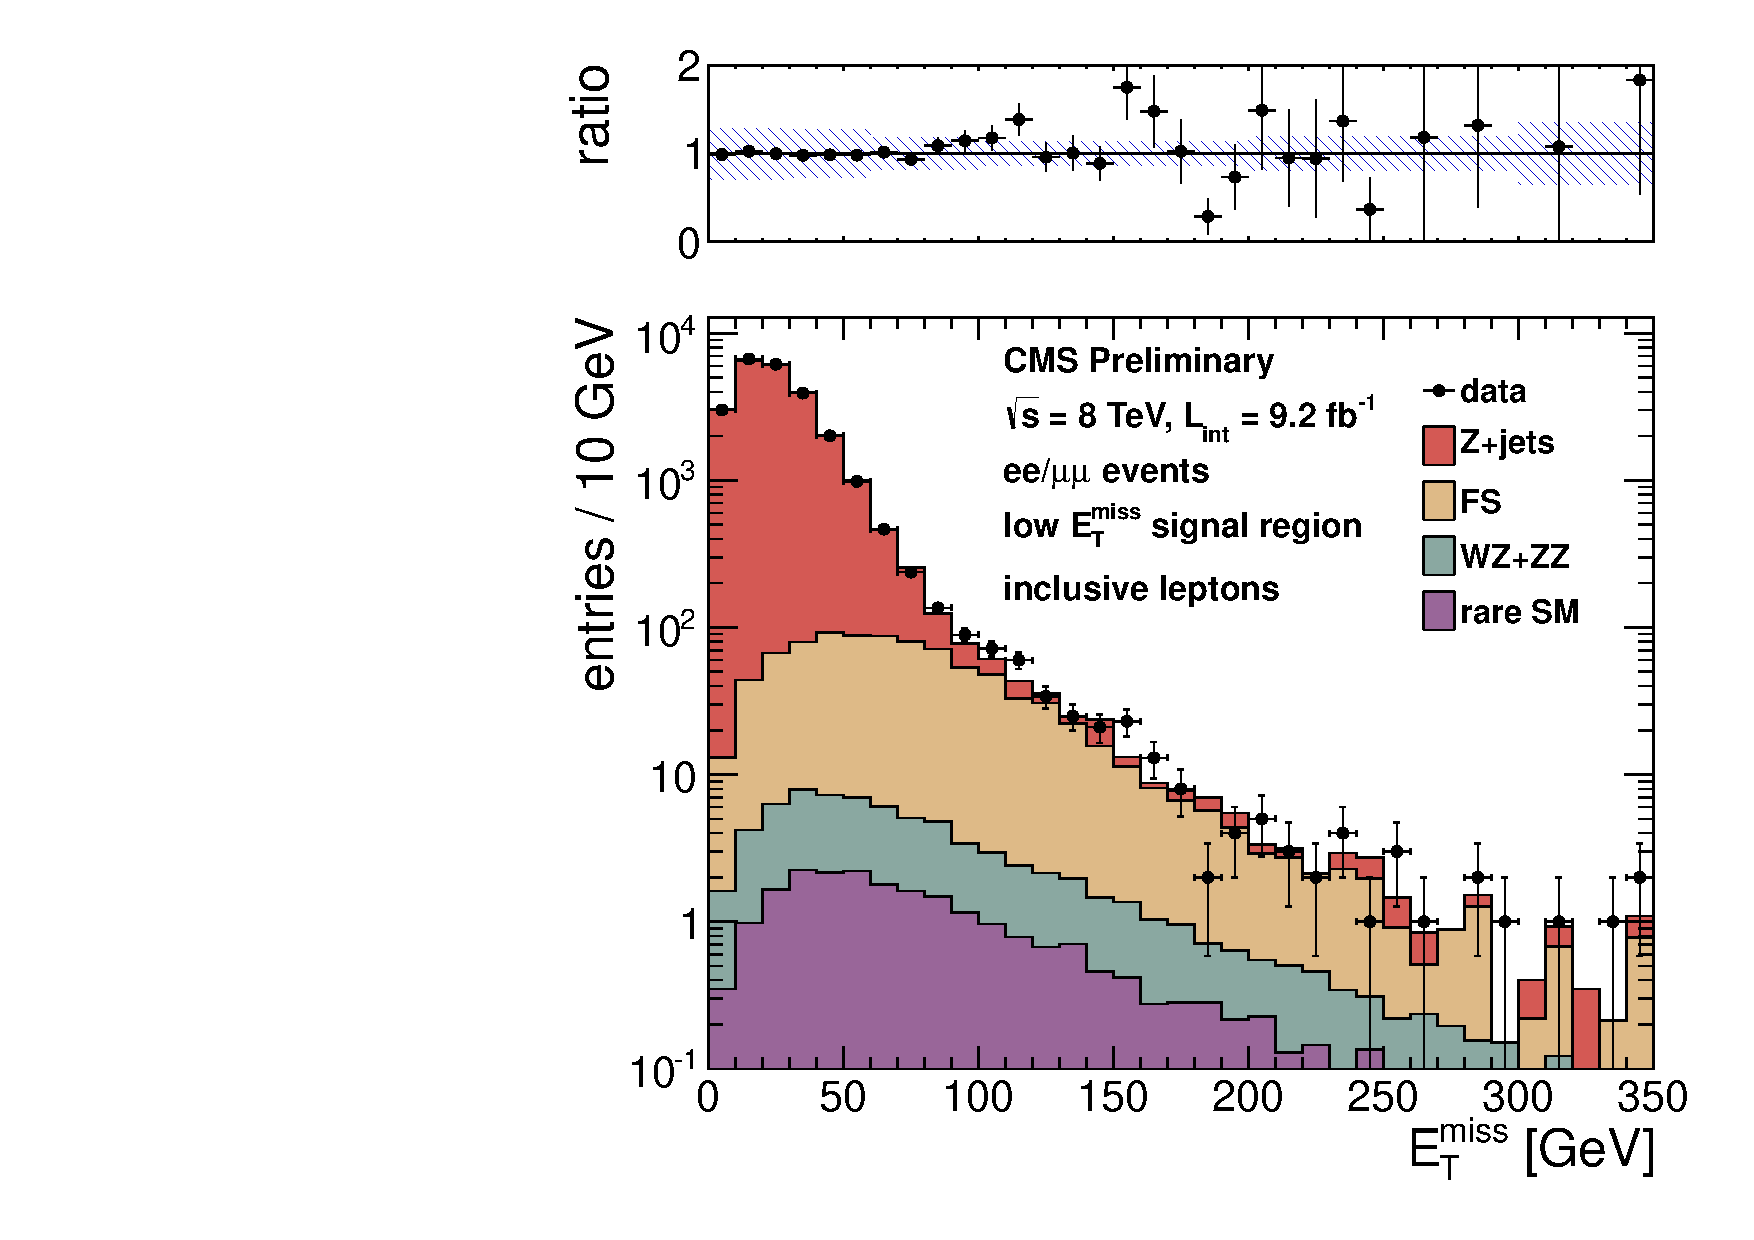
\includegraphics[width=0.45\textwidth]{plots/edge_pfmet_pt40_lowMet_all.pdf}
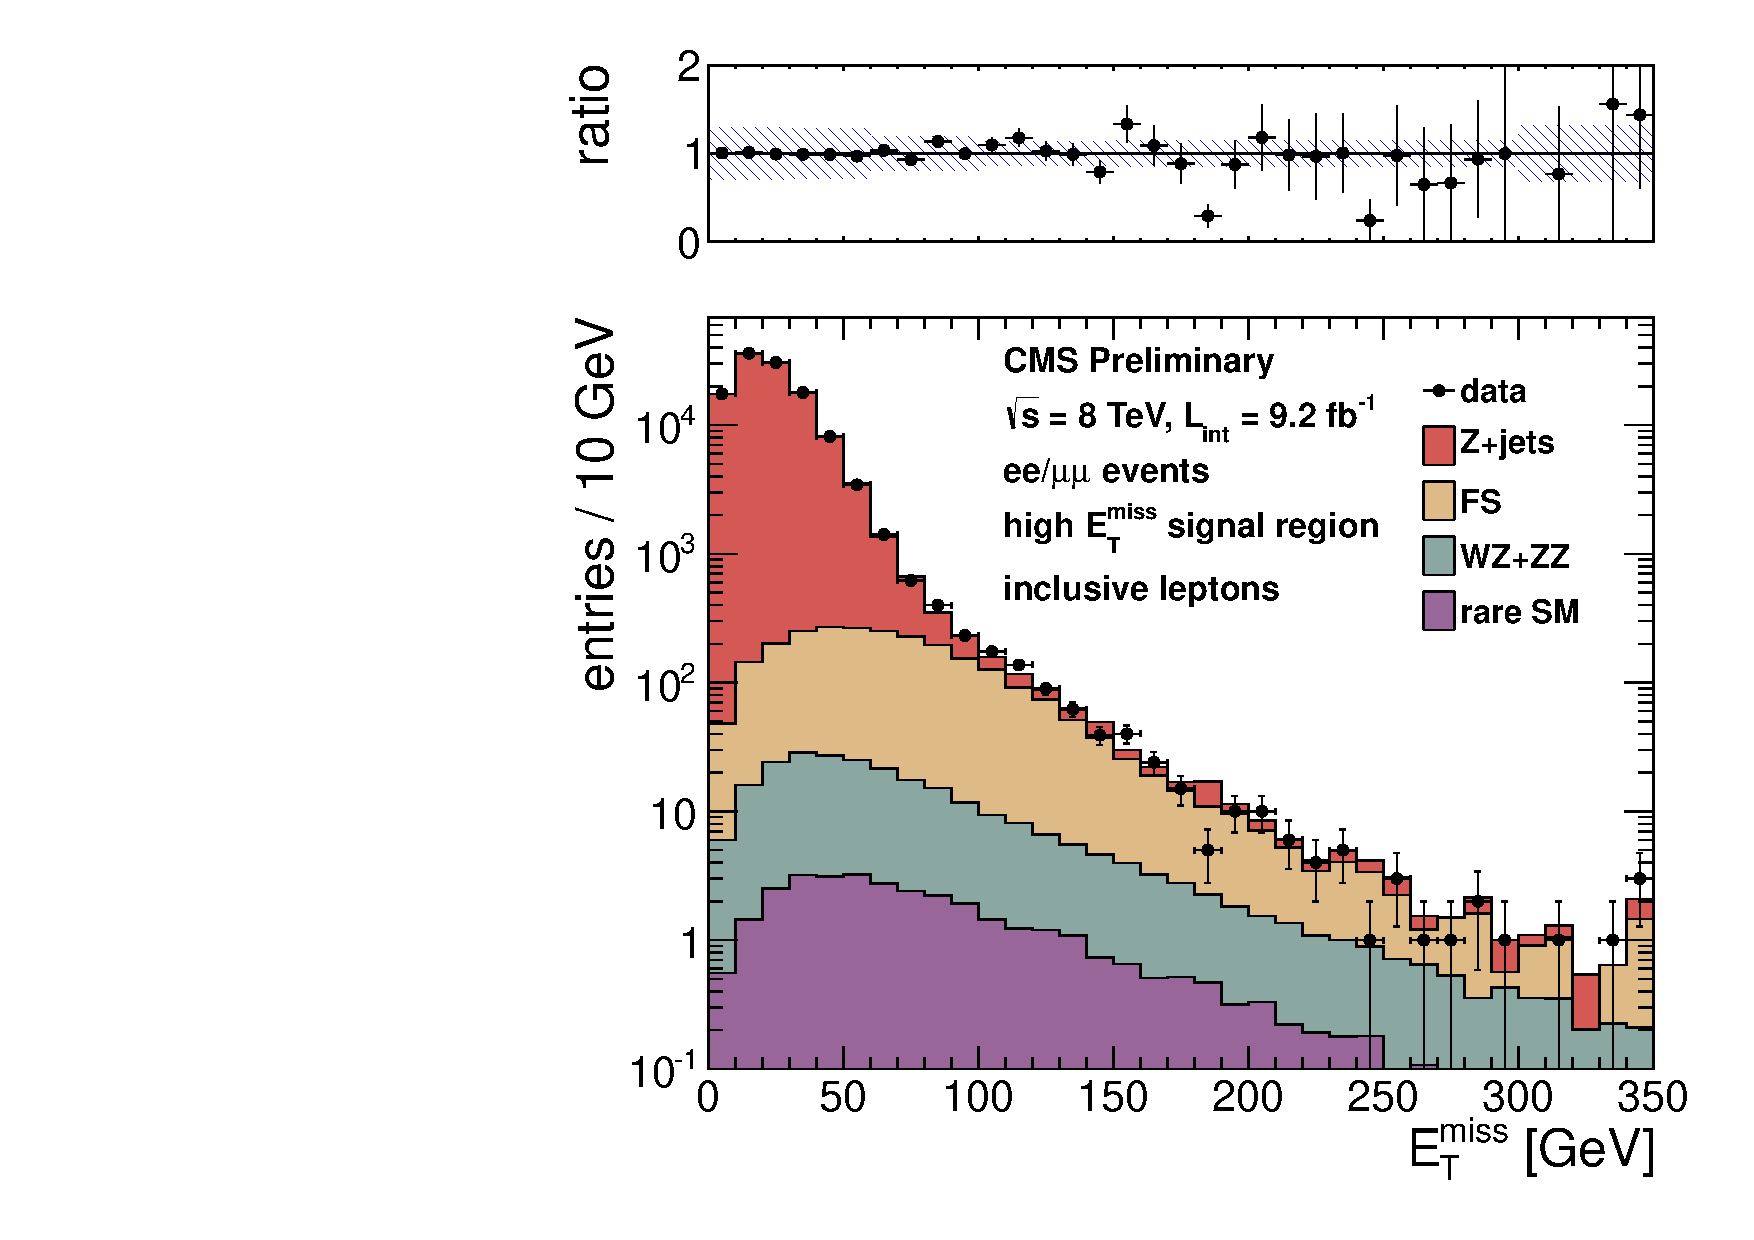
\includegraphics[width=0.45\textwidth]{plots/edge_pfmet_pt40_highMet_all.pdf}
%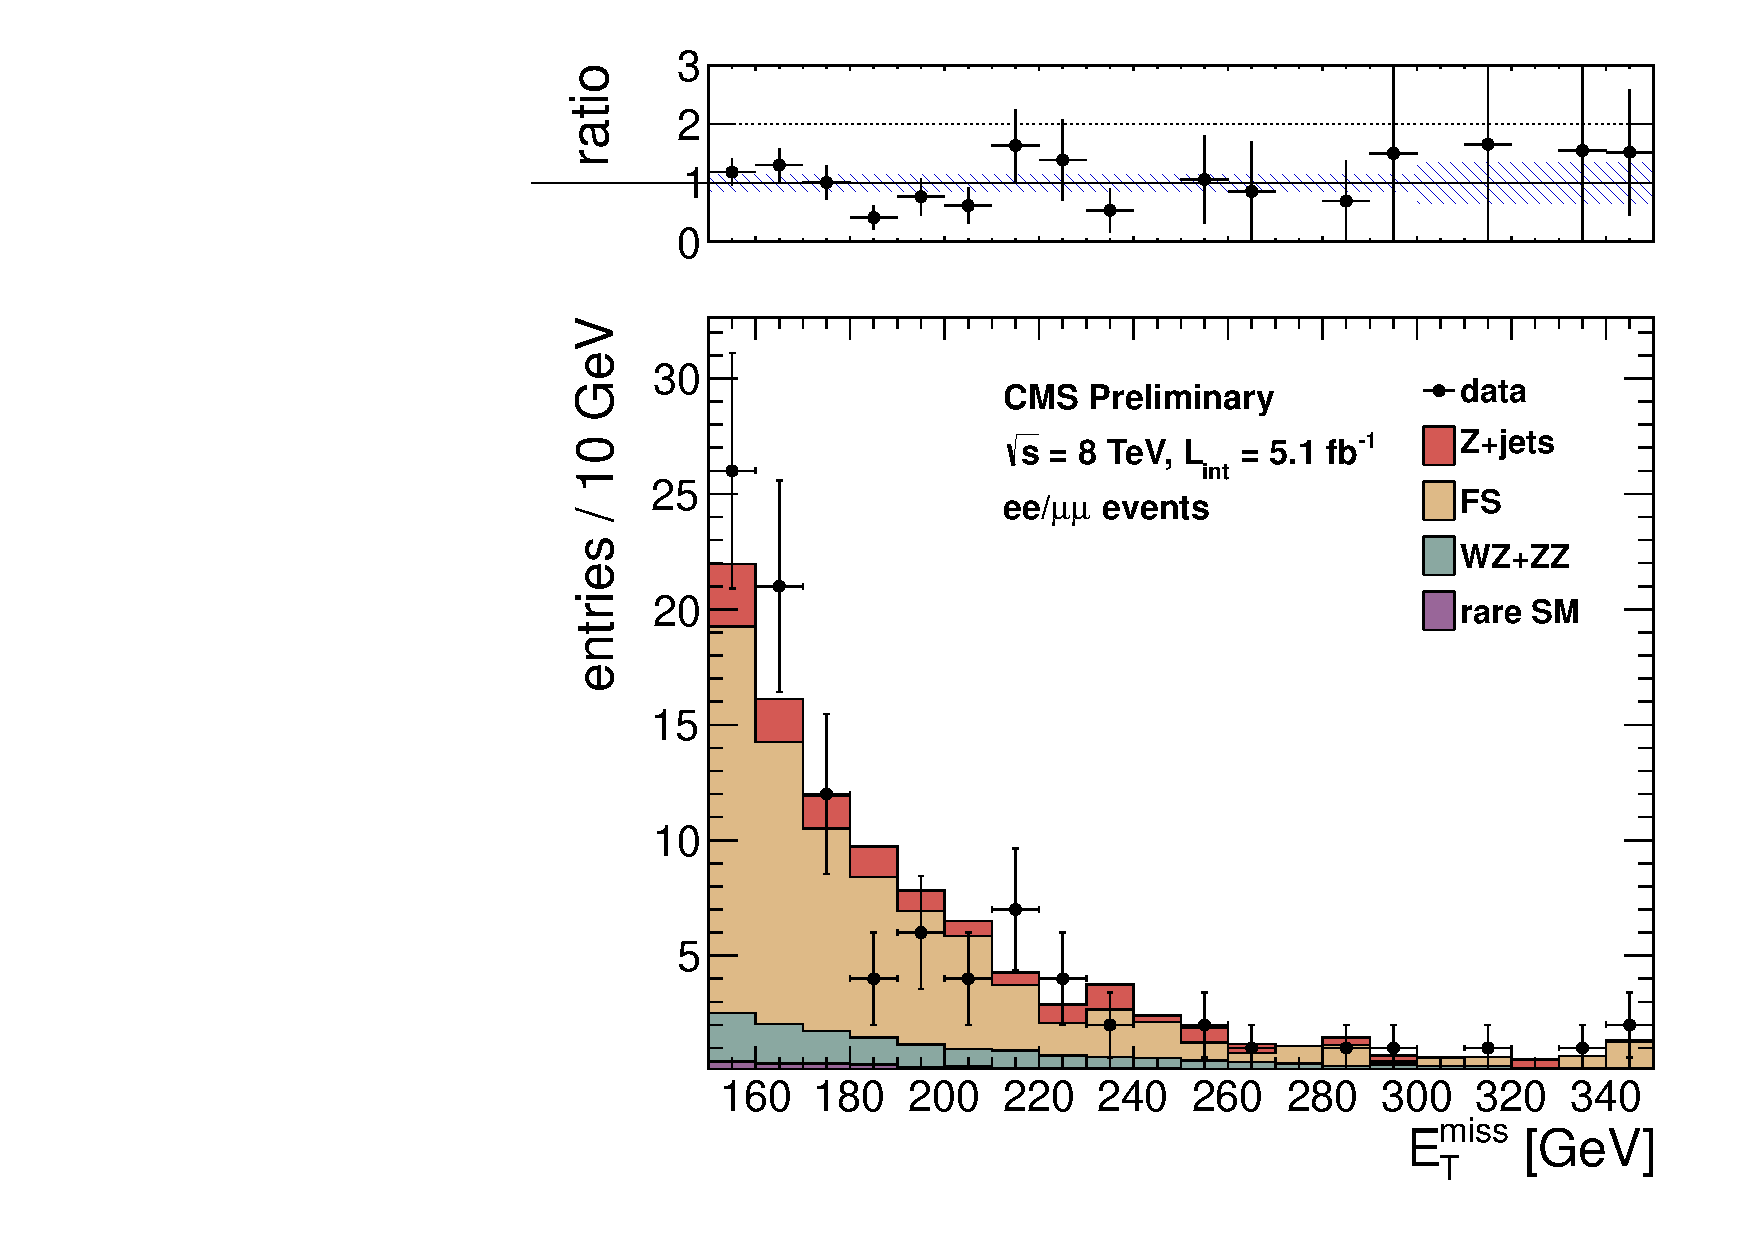
\includegraphics[width=0.48\textwidth]{plots/pfmet_pt40_2012AB_highMet_all_linear.pdf}
\end{tabular}
\caption{\footnotesize {\bf Results of for the low \MET\ (left) and high \MET\ (right) signal regions with the inclusive lepton selection.}
The observed \MET\ distribution (black points) is compared with the sum of the predicted \MET\
distributions from \zjets, flavor-symmetric backgrounds, WZ+ZZ backgrounds, and rare SM backgrounds. 
The ratio of observed to predicted yields in each bin is
indicated. The error bars indicate the statistical uncertainty in the data and the shaded band indicates the total background uncertainty.
\label{fig:results_inclusive}
}
\end{center}
\end{figure}

\begin{table}[htb]
\begin{center}
\footnotesize
\caption{\label{tab:results_inclusive}\footnotesize {\bf Results for the low \MET\ signal region (top table) and high \MET\ signal region (bottom table) with the inclusive lepton selection.} 
The total background is the sum of the \zjets\ background predicted from
the \MET\ templates method (\zjets\ bkg), the flavor-symmetric background predicted from e$\mu$ events (FS bkg), the WZ and ZZ backgrounds predicted from MC
(WZ bkg and ZZ bkg) and the rare SM backgrounds. All uncertainties include both the statistical and systematic components. The Gaussian significance of the deviation between the data 
and total background is indicated for signal regions with at least 20 observed events. }
\begin{tabular}{l|c|c|c|c|c|c}

\hline
\hline

\begin{comment}
Using pfmet out-of-the-box
NEED TO RE-EVALUATE K!!!!!!!!!!!!!!!!!
Using pT > 40 GeV jets, low MET signal region
WZ/ZZ selection : ((((((leptype==0 && (ee==1 || isdata==0))||(leptype==1 && (mm==1 || isdata==0)))&&(ngennu>0))&&(csc==0 && hbhe==1 && hcallaser==1 && ecaltp==1 && trkfail==1 && eebadsc==1 && hbhenew==1))&&(dilmass>81 && dilmass<101))&&(lep1.pt()>20.0 && lep2.pt()>20.0))&&(njets40>=3)
WZ/ZZ weight    : weight * 9.2 * vtxweight * trgeff
Opening ../output/V00-01-04/babylooper_edge_data_ALL_53X_PhotonStitchedTemplate_pfmet_pt40_lowMet.root
B-veto?   0
K         0.14
ee+mm channels: scale em yield by 0.99
Yields in 0-60 GeV region
data   : 22782
gjets  : 23299
OF     : 350.242
WZ     : 22.2641
ZZ     : 2.36791
Rare   : 9.60548
Scaling gjets by : 0.961309
SF events 23999
OF events 5826

ee/#mu#mu events
\end{comment}

                      &   \MET\ $>$ 0 GeV   &  \MET\ $>$ 30 GeV   &  \MET\ $>$ 60 GeV   & \MET\ $>$ 100 GeV   & \MET\ $>$ 150 GeV   & \MET\ $>$ 300 GeV  \\
\hline
        \zjets\ bkg   &  23071 $\pm$ 6922   &   7456 $\pm$ 2238   &     673 $\pm$ 203   &   49.9 $\pm$ 16.4   &    10.4 $\pm$ 3.6   &     1.0 $\pm$ 0.6  \\
             FS bkg   &     807 $\pm$ 126   &     695 $\pm$ 108   &      457 $\pm$ 71   &      184 $\pm$ 29   &    45.6 $\pm$ 7.5   &     1.5 $\pm$ 0.5  \\
             WZ bkg   &   43.5 $\pm$ 30.5   &   35.1 $\pm$ 24.6   &   21.3 $\pm$ 14.9   &    10.0 $\pm$ 7.1   &     4.4 $\pm$ 3.2   &     0.4 $\pm$ 0.4  \\
             ZZ bkg   &     7.8 $\pm$ 3.9   &     7.0 $\pm$ 3.6   &     5.4 $\pm$ 2.8   &     3.3 $\pm$ 1.8   &     1.7 $\pm$ 1.1   &     0.2 $\pm$ 0.2  \\
        rare SM bkg   &   22.0 $\pm$ 11.0   &    19.0 $\pm$ 9.6   &    12.4 $\pm$ 6.3   &     6.3 $\pm$ 3.3   &     2.8 $\pm$ 1.6   &     0.3 $\pm$ 0.3  \\
\hline
          total bkg   &  23951 $\pm$ 6924   &   8213 $\pm$ 2241   &    1169 $\pm$ 216   & {\bf     253 $\pm$ 34 }  &    64.8 $\pm$ 9.1   &     3.5 $\pm$ 1.0  \\
               data   &             23999   &              8134   &              1217   & {\bf          288 }      &                76   &                 4  \\
       significance   &       0.0$\sigma$   &      -0.0$\sigma$   &       0.2$\sigma$   & {\bf      0.9$\sigma$ }  &       0.9$\sigma$   &                    \\
\hline
\hline

\begin{comment}
Using pfmet out-of-the-box
NEED TO RE-EVALUATE K!!!!!!!!!!!!!!!!!
Using pT > 40 GeV jets, high MET signal region
WZ/ZZ selection : (((((((leptype==0 && (ee==1 || isdata==0))||(leptype==1 && (mm==1 || isdata==0)))&&(ngennu>0))&&(csc==0 && hbhe==1 && hcallaser==1 && ecaltp==1 && trkfail==1 && eebadsc==1 && hbhenew==1))&&(dilmass>81 && dilmass<101))&&(lep1.pt()>20.0 && lep2.pt()>20.0))&&(njets40>=2))&&(ht40>=100.0)
WZ/ZZ weight    : weight * 9.2 * vtxweight * trgeff
Opening ../output/V00-01-04/babylooper_edge_data_ALL_53X_PhotonStitchedTemplate_pfmet_pt40_highMet.root
B-veto?   0
K         0.14
ee+mm channels: scale em yield by 0.99
Yields in 0-60 GeV region
data   : 113677
gjets  : 115027
OF     : 1054.05
WZ     : 100.866
ZZ     : 11.955
Rare   : 14.0179
Scaling gjets by : 0.978
SF events 116978
OF events 16270

ee/#mu#mu events
\end{comment}

                      &   \MET\ $>$ 0 GeV   &  \MET\ $>$ 30 GeV   &  \MET\ $>$ 60 GeV   & \MET\ $>$ 100 GeV   & \MET\ $>$ 150 GeV   & \MET\ $>$ 300 GeV  \\
\hline
        \zjets\ bkg   &114401 $\pm$ 34322   &  30966 $\pm$ 9291   &    1905 $\pm$ 573   &      120 $\pm$ 38   &    26.2 $\pm$ 8.9   &     1.4 $\pm$ 0.7  \\
             FS bkg   &    2255 $\pm$ 350   &    1908 $\pm$ 296   &    1201 $\pm$ 187   &      436 $\pm$ 68   &   90.0 $\pm$ 14.4   &     2.9 $\pm$ 0.8  \\
             WZ bkg   & 182.7 $\pm$ 127.9   & 144.7 $\pm$ 101.3   &   81.8 $\pm$ 57.3   &   35.2 $\pm$ 24.7   &    13.9 $\pm$ 9.9   &     1.3 $\pm$ 1.3  \\
             ZZ bkg   &   35.9 $\pm$ 18.0   &   32.3 $\pm$ 16.2   &   23.9 $\pm$ 12.0   &    14.0 $\pm$ 7.1   &     6.7 $\pm$ 3.6   &     0.8 $\pm$ 0.8  \\
        rare SM bkg   &   33.5 $\pm$ 16.8   &   29.0 $\pm$ 14.6   &    19.5 $\pm$ 9.8   &    10.2 $\pm$ 5.2   &     4.5 $\pm$ 2.5   &     0.5 $\pm$ 0.5  \\
\hline
          total bkg   &116908 $\pm$ 34324   &  33080 $\pm$ 9296   &    3231 $\pm$ 605   &      616 $\pm$ 82   & {\bf     141 $\pm$ 20 }  &     6.9 $\pm$ 1.9  \\
               data   &            116978   &             32796   &              3301   &               635   & {\bf              133 }  &                 5  \\
       significance   &       0.0$\sigma$   &      -0.0$\sigma$   &       0.1$\sigma$   &       0.2$\sigma$   & {\bf     -0.4$\sigma$ }  &                    \\

\hline
\hline

\end{tabular}
\end{center}
\end{table}

\clearpage


\begin{figure}[!h]
\begin{center}
\begin{tabular}{cc}
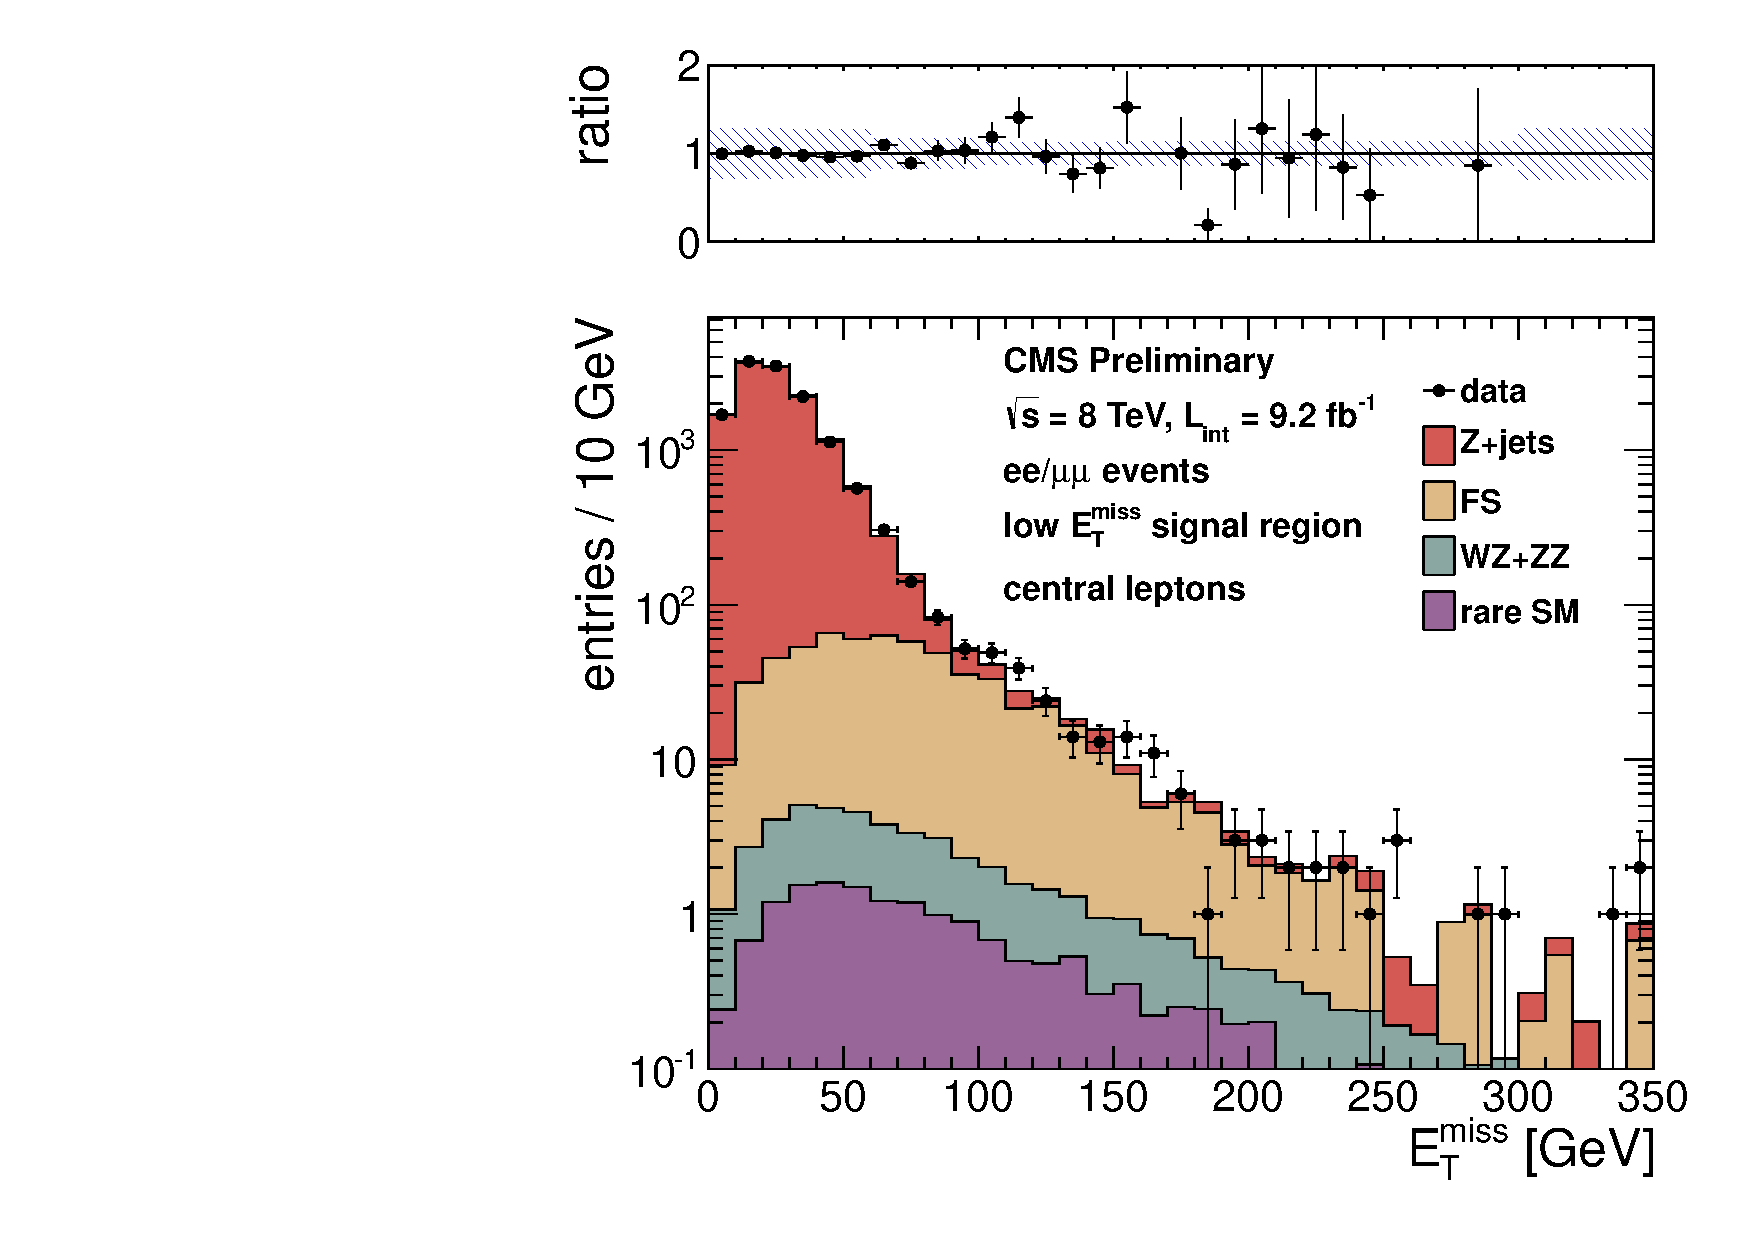
\includegraphics[width=0.45\textwidth]{plots/edge_pfmet_pt40_lowMet_central_all.pdf}
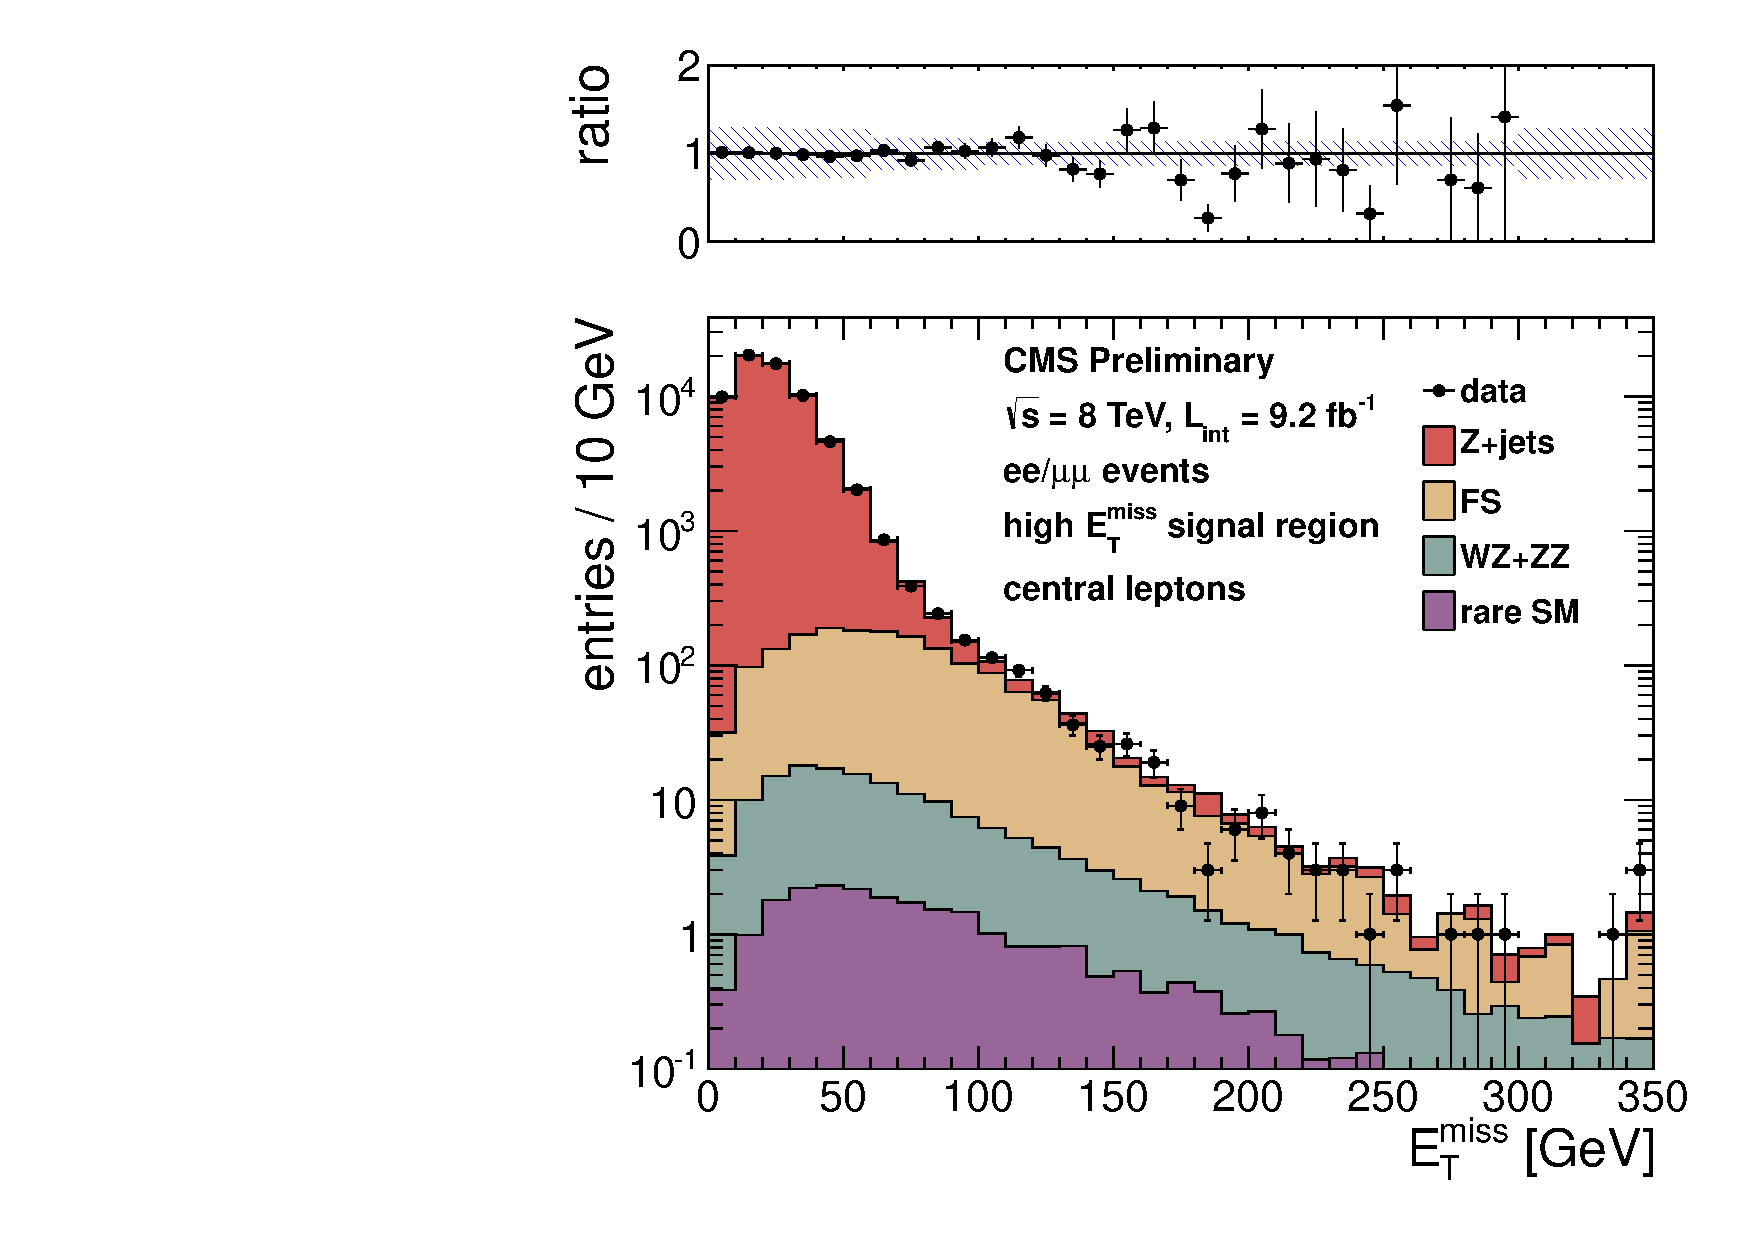
\includegraphics[width=0.45\textwidth]{plots/edge_pfmet_pt40_highMet_central_all.pdf}
%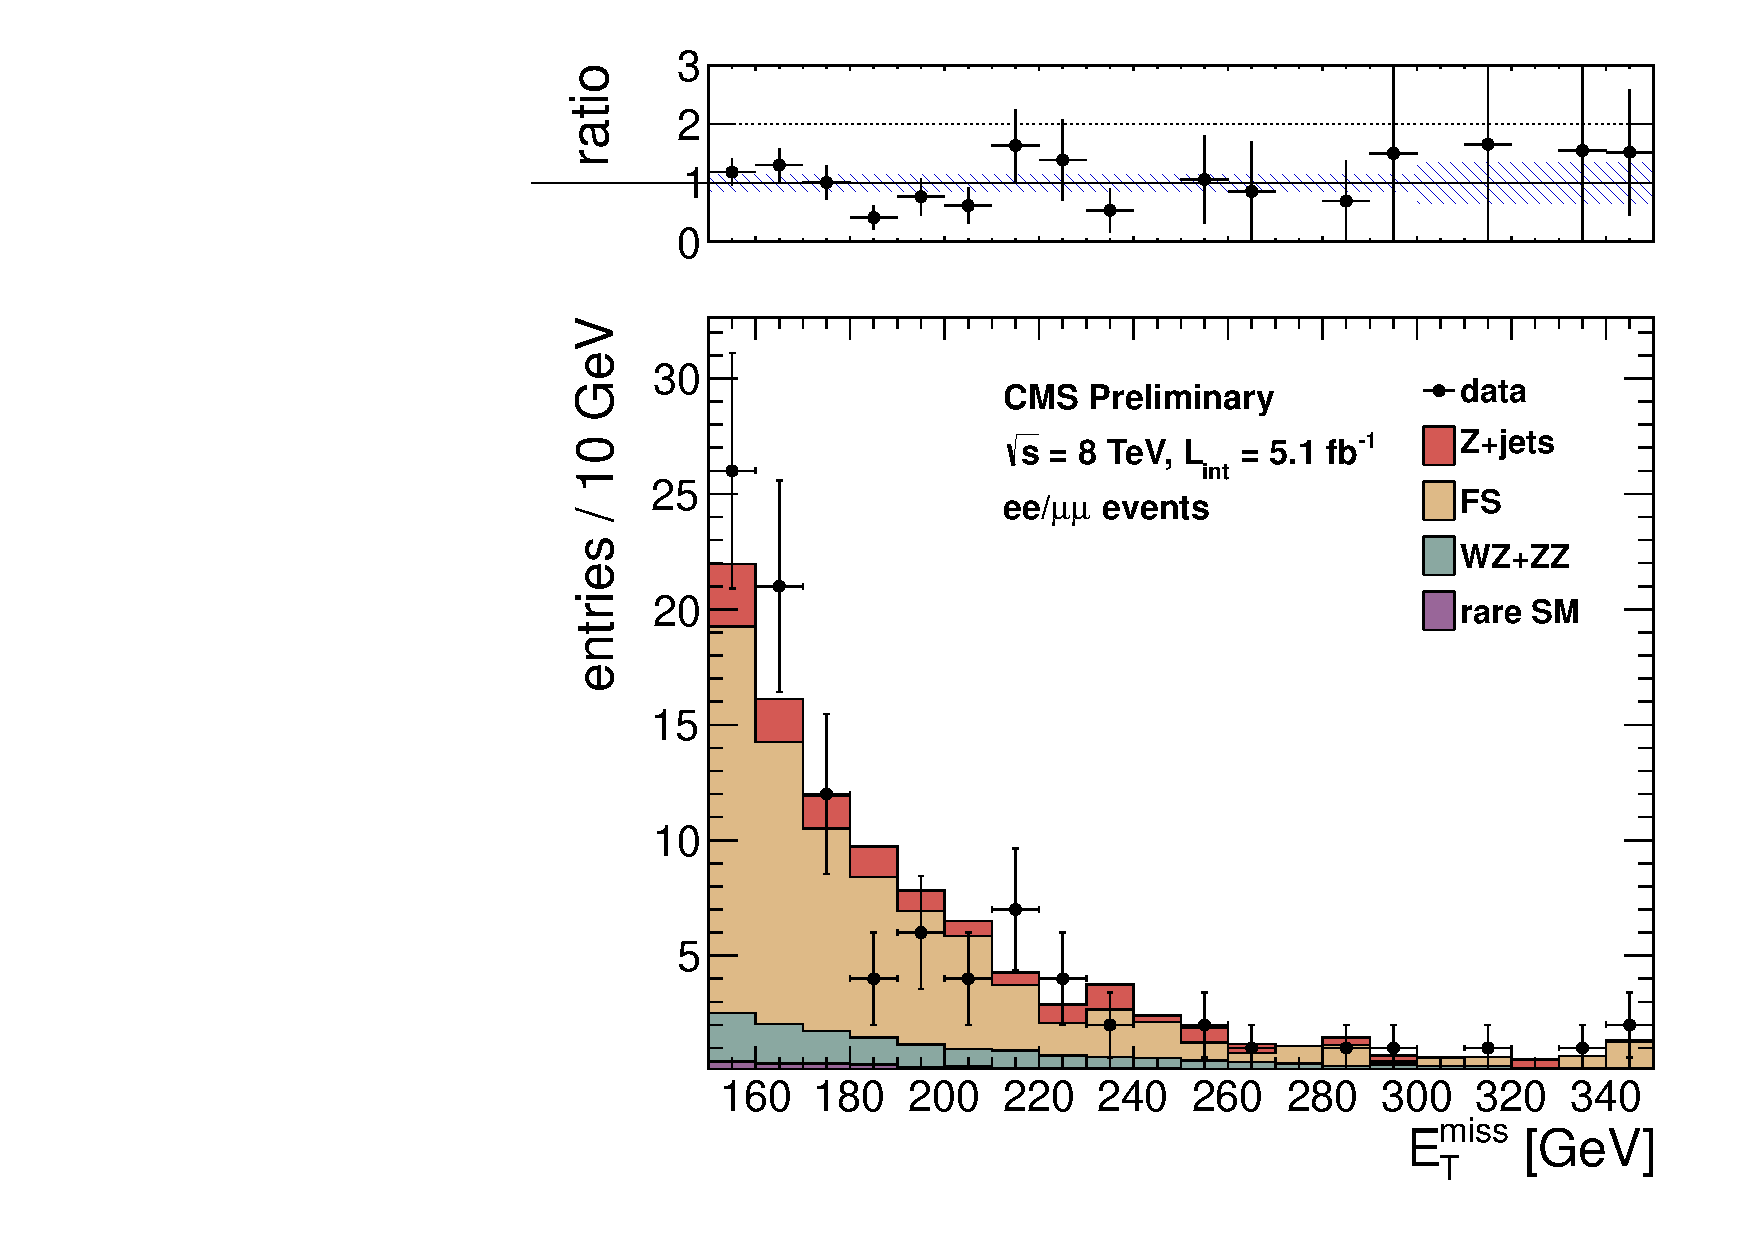
\includegraphics[width=0.48\textwidth]{plots/pfmet_pt40_2012AB_highMet_all_linear.pdf}
\end{tabular}
\caption{\footnotesize {\bf Results of for the low \MET\ (left) and high \MET\ (right) signal regions with the central lepton selection.}
The observed \MET\ distribution (black points) is compared with the sum of the predicted \MET\
distributions from \zjets, flavor-symmetric backgrounds, WZ+ZZ backgrounds, and rare SM backgrounds. 
The ratio of observed to predicted yields in each bin is
indicated. The error bars indicate the statistical uncertainty in the data and the shaded band indicates the total background uncertainty.
\label{fig:results_central}
}
\end{center}
\end{figure}

\begin{table}[htb]
\begin{center}
\footnotesize
\caption{\label{tab:results_central}\footnotesize {\bf Results for the low \MET\ signal region (top table) and high \MET\ signal region (bottom table) with the central lepton selection.} 
The total background is the sum of the \zjets\ background predicted from
the \MET\ templates method (\zjets\ bkg), the flavor-symmetric background predicted from e$\mu$ events (FS bkg), the WZ and ZZ backgrounds predicted from MC
(WZ bkg and ZZ bkg) and the rare SM backgrounds. All uncertainties include both the statistical and systematic components. The Gaussian significance of the deviation between the data 
and total background is indicated for signal regions with at least 20 observed events. }
\begin{tabular}{l|c|c|c|c|c|c}

\hline
\hline

\begin{comment}
Using pfmet out-of-the-box
NEED TO RE-EVALUATE K!!!!!!!!!!!!!!!!!
Using pT > 40 GeV jets, low MET signal region, central leptons
WZ/ZZ selection : (((((((leptype==0 && (ee==1 || isdata==0))||(leptype==1 && (mm==1 || isdata==0)))&&(ngennu>0))&&(csc==0 && hbhe==1 && hcallaser==1 && ecaltp==1 && trkfail==1 && eebadsc==1 && hbhenew==1))&&(dilmass>81 && dilmass<101))&&(lep1.pt()>20.0 && lep2.pt()>20.0))&&(njets40>=3))&&(abs(lep1.eta()) < 1.4 && abs(lep2.eta()) < 1.4)
WZ/ZZ weight    : weight * 9.2 * vtxweight * trgeff
Opening ../output/V00-01-04/babylooper_edge_data_ALL_53X_PhotonStitchedTemplate_pfmet_pt40_lowMet_central.root
B-veto?   0
K         0.15
ee+mm channels: scale em yield by 0.99
Yields in 0-60 GeV region
data   : 12858
gjets  : 13220.3
OF     : 242.649
WZ     : 14.1734
ZZ     : 1.45279
Rare   : 6.75969
Scaling gjets by : 0.952549
SF events 13631
OF events 3806

ee/#mu#mu events
\end{comment}

                      &   \MET\ $>$ 0 GeV   &  \MET\ $>$ 30 GeV   &  \MET\ $>$ 60 GeV   & \MET\ $>$ 100 GeV   & \MET\ $>$ 150 GeV   & \MET\ $>$ 300 GeV  \\
\hline
        \zjets\ bkg   &  12984 $\pm$ 3896   &   4242 $\pm$ 1273   &     391 $\pm$ 118   &    29.6 $\pm$ 9.7   &     6.3 $\pm$ 2.2   &     0.6 $\pm$ 0.4  \\
             FS bkg   &      565 $\pm$ 83   &      487 $\pm$ 72   &      323 $\pm$ 48   &      129 $\pm$ 19   &    32.5 $\pm$ 5.2   &     1.2 $\pm$ 0.5  \\
             WZ bkg   &   28.1 $\pm$ 19.7   &   22.7 $\pm$ 15.9   &    13.9 $\pm$ 9.8   &     6.8 $\pm$ 4.9   &     3.1 $\pm$ 2.4   &     0.4 $\pm$ 0.4  \\
             ZZ bkg   &     4.8 $\pm$ 2.5   &     4.4 $\pm$ 2.3   &     3.3 $\pm$ 1.8   &     2.1 $\pm$ 1.2   &     1.1 $\pm$ 0.8   &     0.1 $\pm$ 0.1  \\
        rare SM bkg   &    15.8 $\pm$ 8.0   &    13.7 $\pm$ 6.9   &     9.0 $\pm$ 4.6   &     4.8 $\pm$ 2.5   &     2.3 $\pm$ 1.4   &     0.3 $\pm$ 0.3  \\
\hline
          total bkg   &  13598 $\pm$ 3897   &   4770 $\pm$ 1275   &     740 $\pm$ 128   &{\bf      173 $\pm$ 22}   &    45.2 $\pm$ 6.3   &     2.6 $\pm$ 0.7  \\
               data   &             13631   &              4688   &               773   &{\bf               192}   &                53   &                 3  \\
       significance   &       0.0$\sigma$   &      -0.1$\sigma$   &       0.3$\sigma$   &{\bf       0.7$\sigma$}   &       0.8$\sigma$   &                    \\
\hline
\hline

\begin{comment}
Using pfmet out-of-the-box
NEED TO RE-EVALUATE K!!!!!!!!!!!!!!!!!
Using pT > 40 GeV jets, high MET signal region, central leptons
WZ/ZZ selection : ((((((((leptype==0 && (ee==1 || isdata==0))||(leptype==1 && (mm==1 || isdata==0)))&&(ngennu>0))&&(csc==0 && hbhe==1 && hcallaser==1 && ecaltp==1 && trkfail==1 && eebadsc==1 && hbhenew==1))&&(dilmass>81 && dilmass<101))&&(lep1.pt()>20.0 && lep2.pt()>20.0))&&(njets40>=2))&&(ht40>=100.0))&&(abs(lep1.eta()) < 1.4 && abs(lep2.eta()) < 1.4)
WZ/ZZ weight    : weight * 9.2 * vtxweight * trgeff
Opening ../output/V00-01-04/babylooper_edge_data_ALL_53X_PhotonStitchedTemplate_pfmet_pt40_highMet_central.root
B-veto?   0
K         0.15
ee+mm channels: scale em yield by 0.99
Yields in 0-60 GeV region
data   : 64459
gjets  : 65372.5
OF     : 722.898
WZ     : 62.6465
ZZ     : 6.86106
Rare   : 9.85893
Scaling gjets by : 0.973755
SF events 66521
OF events 10593

ee/#mu#mu events
\end{comment}

                      &   \MET\ $>$ 0 GeV   &  \MET\ $>$ 30 GeV   &  \MET\ $>$ 60 GeV   & \MET\ $>$ 100 GeV   & \MET\ $>$ 150 GeV   & \MET\ $>$ 300 GeV  \\
\hline
        \zjets\ bkg   & 64775 $\pm$ 19433   &  17697 $\pm$ 5310   &    1118 $\pm$ 336   &   71.8 $\pm$ 22.3   &    15.8 $\pm$ 5.3   &     0.8 $\pm$ 0.4  \\
             FS bkg   &    1573 $\pm$ 231   &    1341 $\pm$ 197   &     850 $\pm$ 125   &      313 $\pm$ 46   &   66.5 $\pm$ 10.2   &     2.2 $\pm$ 0.7  \\
             WZ bkg   &  115.0 $\pm$ 80.5   &   91.3 $\pm$ 64.0   &   52.4 $\pm$ 36.7   &   23.3 $\pm$ 16.4   &     9.4 $\pm$ 6.7   &     1.0 $\pm$ 1.0  \\
             ZZ bkg   &   21.7 $\pm$ 10.9   &    19.7 $\pm$ 9.9   &    14.8 $\pm$ 7.5   &     8.8 $\pm$ 4.5   &     4.3 $\pm$ 2.4   &     0.5 $\pm$ 0.5  \\
        rare SM bkg   &   23.9 $\pm$ 12.0   &   20.8 $\pm$ 10.4   &    14.1 $\pm$ 7.1   &     7.5 $\pm$ 3.9   &     3.6 $\pm$ 2.1   &     0.5 $\pm$ 0.5  \\
\hline
          total bkg   & 66508 $\pm$ 19435   &  19170 $\pm$ 5314   &    2049 $\pm$ 360   &      424 $\pm$ 54   &{\bf   99.6 $\pm$ 13.7}   &     5.1 $\pm$ 1.4  \\
               data   &             66521   &             18841   &              2062   &               421   &{\bf                92}   &                 4  \\
       significance   &       0.0$\sigma$   &      -0.1$\sigma$   &       0.0$\sigma$   &      -0.1$\sigma$   &{\bf      -0.5$\sigma$}   &                    \\
\hline
\hline

\end{tabular}
\end{center}
\end{table}

\clearpage


\subsection{Extrapolation to Low Mass to Estimate the $\gamma^*/Z$ Contribution}

\begin{figure}[t]
\begin{center}
\begin{tabular}{cc}
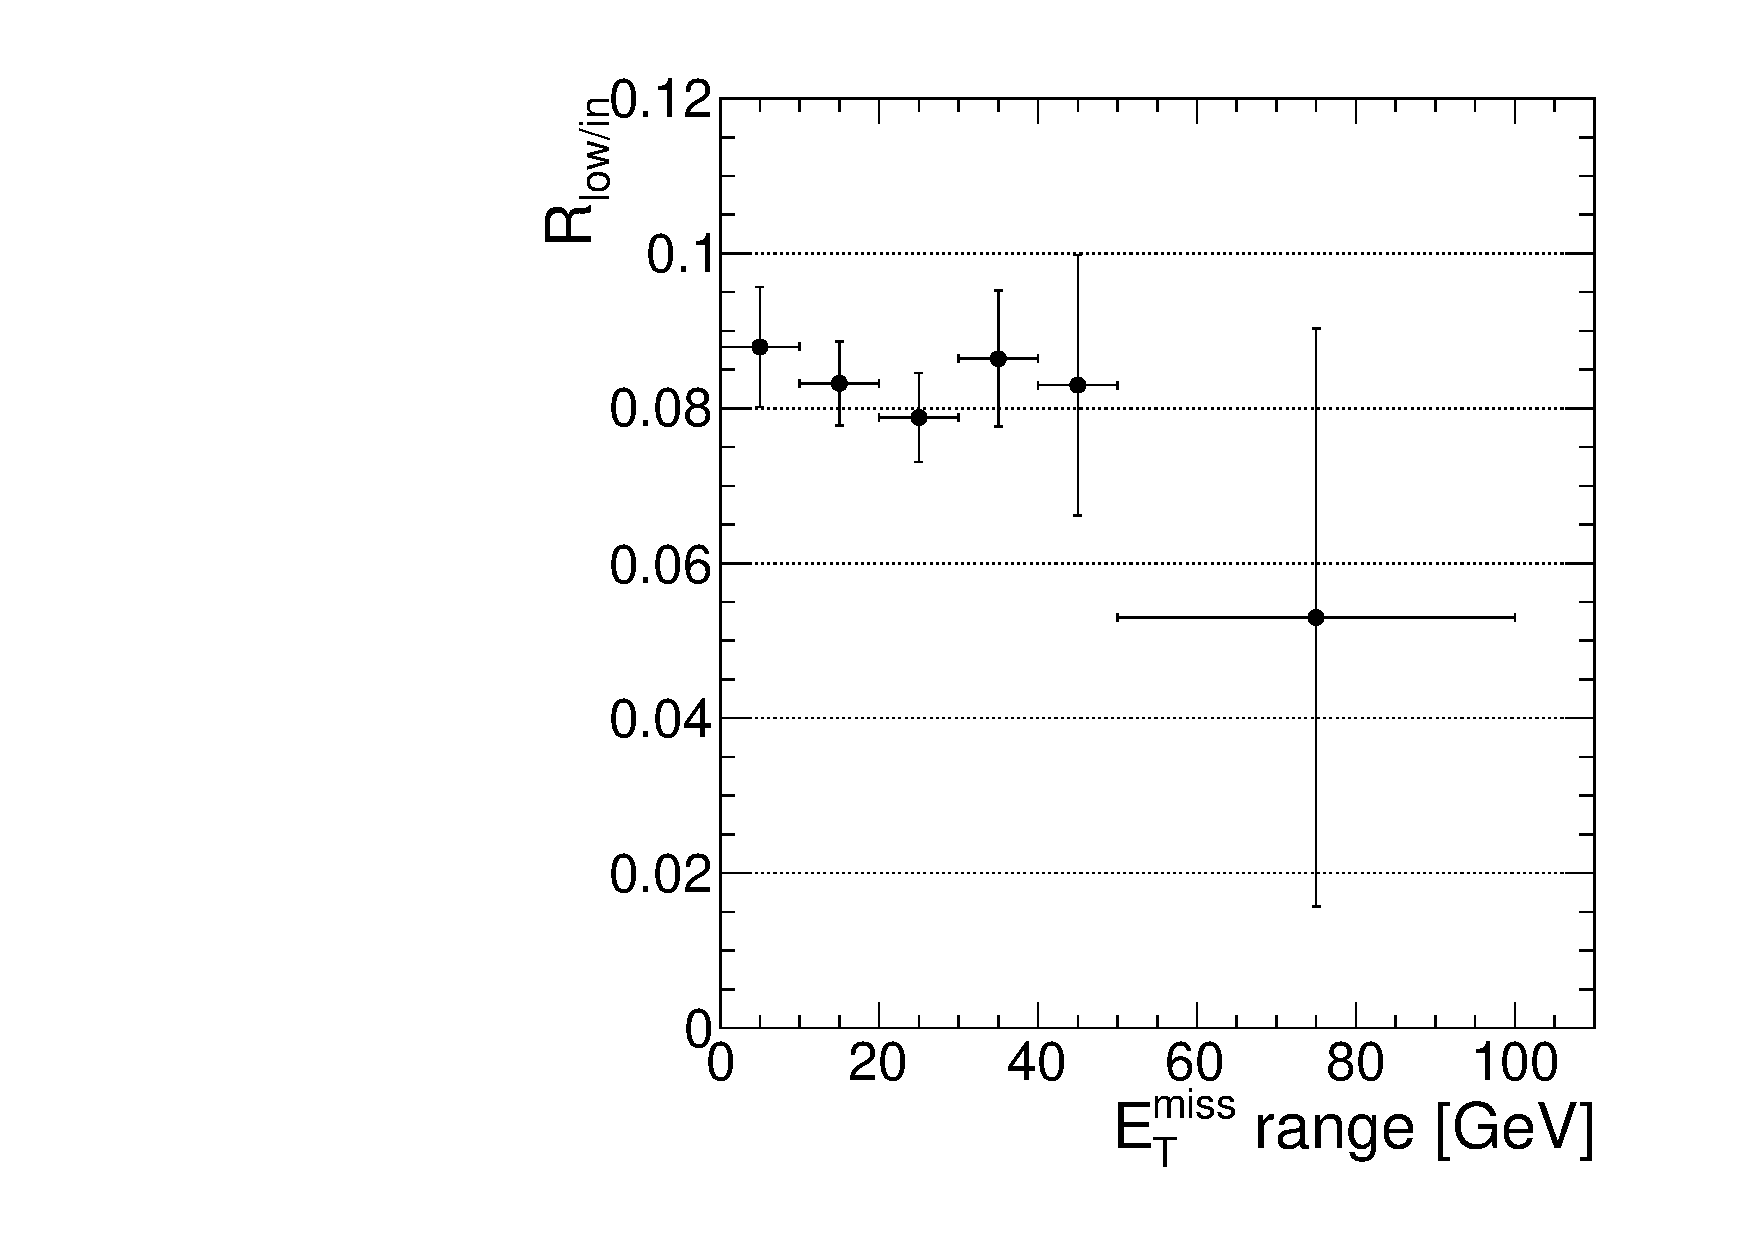
\includegraphics[width=0.4\textwidth]{plots/Routin_lowmet.pdf} &
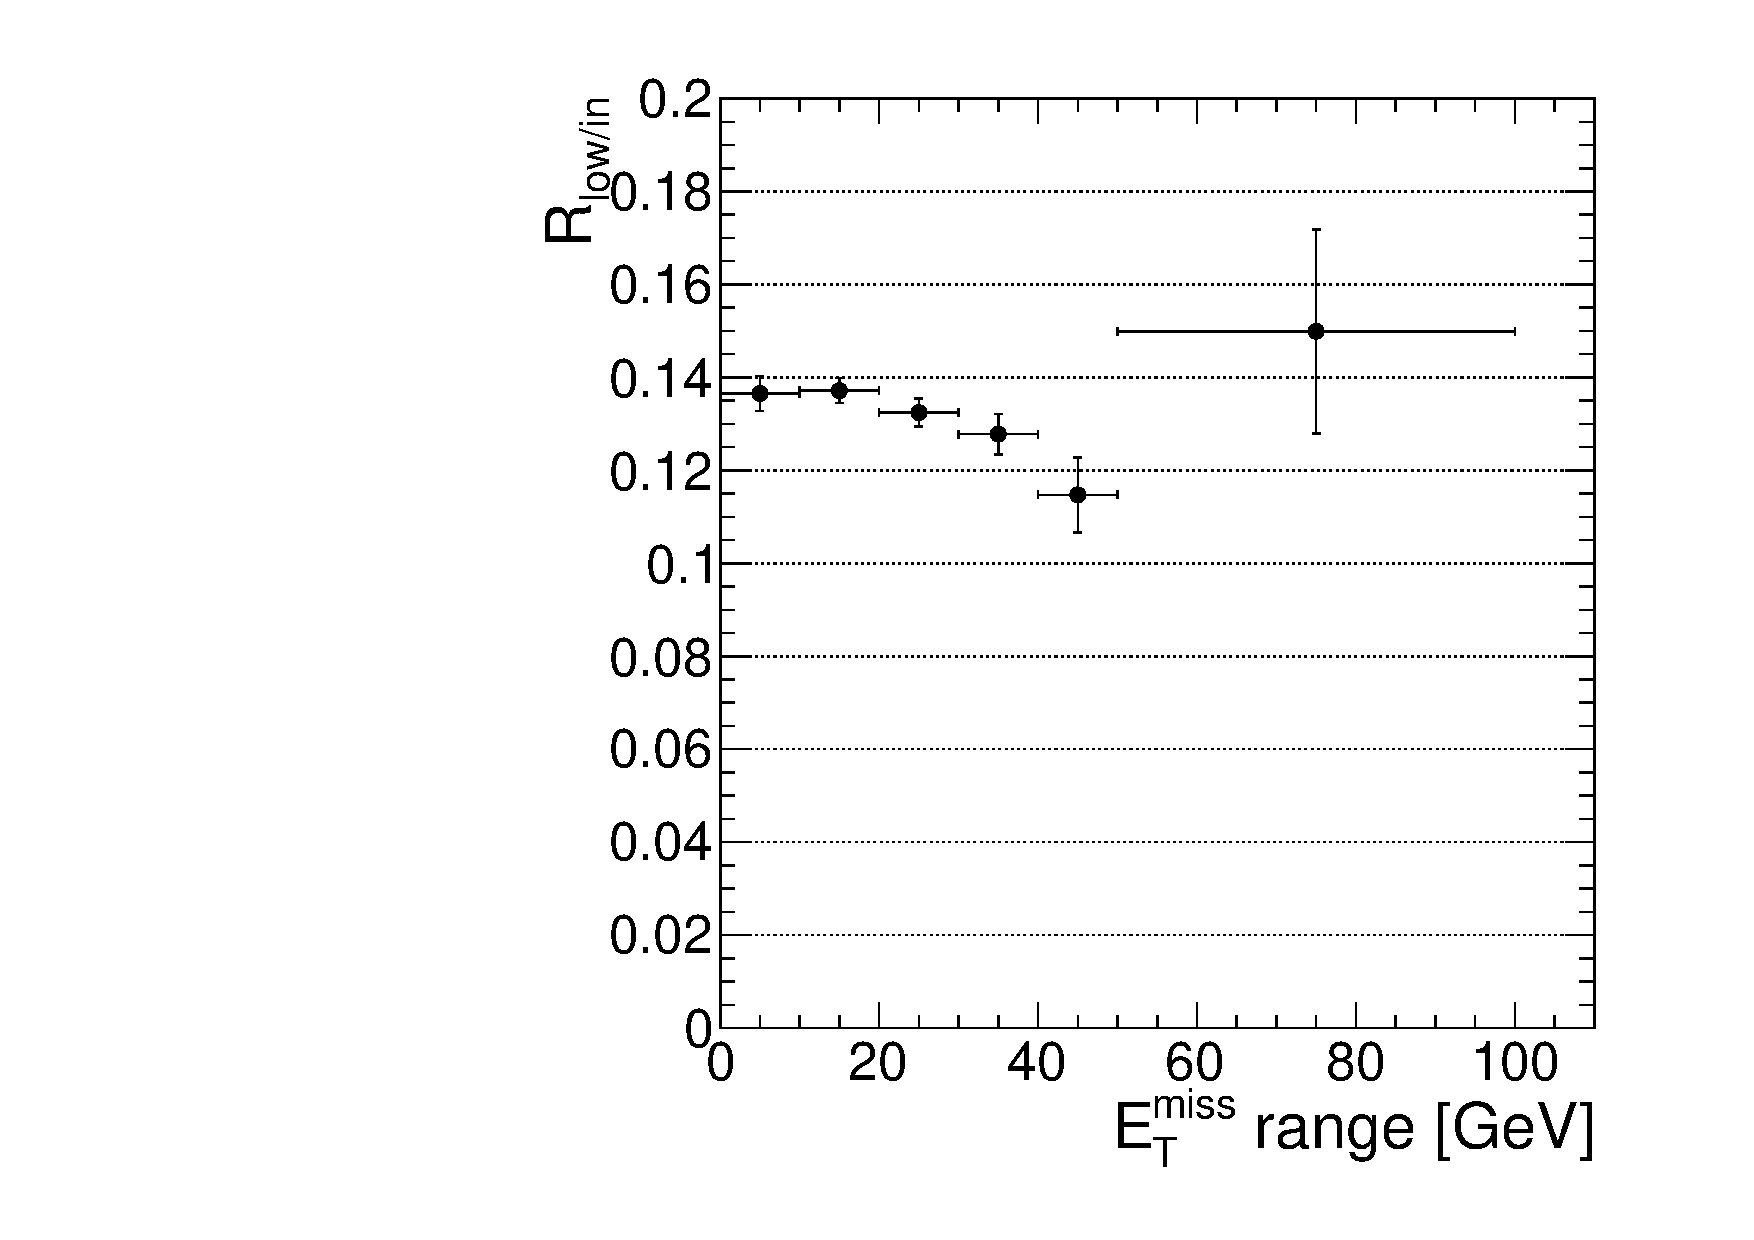
\includegraphics[width=0.4\textwidth]{plots/Routin_highMET.pdf} \\
\end{tabular}
\caption{\label{fig:Routin}
The ratio $R_{low/in}$ of low mass ($15<m_{\ell\ell}<70$ GeV) to on-Z ($81<m_{\ell\ell}<101$ GeV) events, as a function of
the \MET\ requirement. The left plot corresponds to the low \MET\ signal region (2 \pt\ $>$ 20 GeV leptons with at least 3 jets),
the right plot corresponds to the high \MET\ signal region (\pt\ $>$ (20,10) GeV leptons with at least 2 jets). 
}
\end{center}
\end{figure}

Given a prediction for the Z background in the Z mass window, we can extrapolate to estimate the low mass $\gamma^*$/Z contribution.
We extract the ratio $R_{low/in}$ of low-mass  to on-shell Z events from data,
correcting for the contribution from flavor-symmetric backgrounds, according to:

\begin{equation}
R_{low/in} = (N_{SF}^{low}-N_{OF}^{low})/(N_{SF}^{in}-N_{OF}^{in}).
\end{equation}

Here SF and OF refer to the same-flavor and opposite-flavor data yields in the ``low'' ($15<m_{\ell\ell}<70$ GeV) and ``in'' 
($81<m_{\ell\ell}<101$ GeV) dilepton mass regions. To predict the low-mass $\gamma^*$/Z contribution, we scale the total predicted
Z background by this quantity, which is displayed in Fig.~\ref{fig:Routin}. Here we measure $R_{low/in}$ in several \MET\ regions,
and assess the uncertainty based on the variation with respect to \MET. 
Based on this plot we choose $R_{low/in}=0.08\pm0.02$ for the low \MET\ signal region and $R_{low/in}=0.13\pm0.03$ for the high \MET\ region.

We find the following results for the first 5.1 fb$^{-1}$. For the low \MET\ signal region, the total predicted Z background in the Z mass region is $39\pm9.6$ 
(sum of the \zjets, WZ+ZZ, and rare SM backgrounds from Table~\ref{tab:results_lowmet}, \MET\ $>$ 100 GeV region), 
resulting in a $\gamma^*$/Z prediction of $3.1\pm1.1$ events. 
For the high \MET\ signal region, the total predicted Z background in the Z mass region is $30\pm8.1$ 
(sum of the \zjets, WZ+ZZ, and rare SM backgrounds from Table~\ref{tab:results_highmet}, \MET\ $>$ 150 GeV region), 
resulting in a $\gamma^*$/Z prediction of $3.8\pm1.4$ events. 

We find the following results for the full 9.2 fb$^{-1}$. For the low \MET\ signal region, the total predicted Z background in the Z mass region is $68\pm17$ 
(sum of the \zjets, WZ+ZZ, and rare SM backgrounds from Table~\ref{tab:results_edgefull}, \MET\ $>$ 100 GeV region), 
resulting in a $\gamma^*$/Z prediction of $5.4\pm1.9$ events. 
For the high \MET\ signal region, the total predicted Z background in the Z mass region is $60\pm16$ 
(sum of the \zjets, WZ+ZZ, and rare SM backgrounds from Table~\ref{tab:results_edgefull}, \MET\ $>$ 150 GeV region), 
resulting in a $\gamma^*$/Z prediction of $7.9\pm2.7$ events. 

\clearpage

\subsection{Summary of Results}
\label{sec:templates_summary}

In this section we summarize the results for the 5.1 fb$^{-1}$ Run2012A+B data (Table~\ref{tab:results_5p1})
and the 9.2 fb$^{-1}$ Run2012A+B+C data (Table~\ref{tab:results_9p2}).

\begin{table}[htb]
\begin{center}
\caption{\label{tab:results_5p1} Summary of results in 5.1 fb$^{-1}$ 2012A+B data for the low-\MET\ and high-\MET\ signal regions (SR).
In the Z mass region, the predicted Z background (Z bkg, sum of \zjets, WZ/ZZ, and rare SM processes with Z bosons), flavor-symmetric
background (FS bkg), and total background (Total bkg) are indicated, and compared to the observed yield (Data). 
The Gaussian significance of the difference between the data and the total background is indicated.
The predicted $\gamma^*/Z$ contribution to the low-mass region (Low mass $\gamma^*/Z$ bkg) is also indicated.}
\begin{tabular}{l|c|c}

\hline
\hline
& Low-\MET\ SR & High-\MET SR \\
\hline              
Z bkg                        & $39\pm9.6$          & $30\pm8.1$        \\
FS bkg                       & $99\pm16$           & $69\pm12$         \\
Total bkg                    & $138\pm18$          & $98\pm14$         \\
Data                         & 175                 & 95                \\
Significance                 & $+1.6\sigma$        & $-0.2\sigma$      \\
Low mass $\gamma^*/Z$ bkg    & $3.1\pm1.1$         &   $3.8\pm1.4$     \\
\hline
\hline

\end{tabular}
\end{center}
\end{table}

\begin{table}[htb]
\begin{center}
\caption{\label{tab:results_9p2} Summary of results in 9.2 fb$^{-1}$ 2012A+B+C data for the low-\MET\ and high-\MET\ signal regions (SR).
In the Z mass region, the predicted Z background (Z bkg, sum of \zjets, WZ/ZZ, and rare SM processes with Z bosons), flavor-symmetric
background (FS bkg), and total background (Total bkg) are indicated, and compared to the observed yield (Data). 
The Gaussian significance of the difference between the data and the total background is indicated.
The predicted $\gamma^*/Z$ contribution to the low-mass region (Low mass $\gamma^*/Z$ bkg) is also indicated.}
\begin{tabular}{l|c|c}

\hline
\hline
& Low-\MET\ SR & High-\MET SR \\
\hline              
Z bkg                        & $68\pm17$           & $60\pm16$         \\
FS bkg                       & $184\pm29$          & $117\pm20$        \\
Total bkg                    & $251\pm33$          & $177\pm25$        \\
Data                         & 288                 & 167               \\
Significance                 & $+1.0\sigma$        & $-0.4\sigma$      \\
Low mass $\gamma^*/Z$ bkg    & $5.4\pm1.9$         &   $7.9\pm2.7$     \\
\hline
\hline

\end{tabular}
\end{center}
\end{table}


\begin{comment}
The 5.1 fb$^{-1}$ results are summarized as:

\begin{itemize}
\item Low \MET\ signal region
\begin{itemize}
  \item Predicted Z background in Z mass region: $39\pm 9.6$ events
  \item Total predicted background in Z mass region: $138\pm18$ events
  \item Total observed yield in Z mass region: 175 events ($+1.6\sigma$)
  \item Low-mass $\gamma^*$/Z prediction: $3.1\pm1.1$ events
\end{itemize}
\item High \MET\ signal region
\begin{itemize}
  \item Predicted Z background in Z mass region: $30\pm 8.1$ events
  \item Total predicted background in Z mass region: $98\pm14$ events
  \item Total observed yield in Z mass region: 95 events ($-0.2\sigma$)
  \item Low-mass $\gamma^*$/Z prediction: $3.8\pm1.4$ events
\end{itemize}
\end{itemize}


The 9.2 fb$^{-1}$ results are summarized as:

\begin{itemize}
\item Low \MET\ signal region
\begin{itemize}
  \item Predicted Z background in Z mass region: $68\pm17$ events
  \item Total predicted background in Z mass region: $251\pm33$ events
  \item Total observed yield in Z mass region: 288 events ($+1.0\sigma$)
  \item Low-mass $\gamma^*$/Z prediction: $5.4\pm1.9$ events
\end{itemize}
\item High \MET\ signal region
\begin{itemize}
  \item Predicted Z background in Z mass region: $60\pm16$ events
  \item Total predicted background in Z mass region: $177\pm25$ events
  \item Total observed yield in Z mass region: 167 events ($-0.4\sigma$)
  \item Low-mass $\gamma^*$/Z prediction: $7.9\pm2.7$ events
\end{itemize}
\end{itemize}

\end{comment}

\clearpage



\clearpage
\section{Cross-check with single lepton triggers}
\label{sec:triggers}

{\bf The results in this section are based on the old definitions of the high-\MET\ and low-\MET\ signal regions. The high-\MET\ signal region has \pt\ $>$ (20,10) GeV leptons. The low-\MET\ signal region has inclusive leptons.}
The nominal ``edge analysis'' is performed with dilepton triggers. An excess of SF vs. OF events may thus be observed if there
were some inefficiency for the e$\mu$ triggers used in this analysis. In this section we provide a cross-check of the nominal
analysis by including events collected with single lepton triggers. The relevant triggers are:

\begin{itemize}

\item ee channel
\begin{itemize}
\item dilepton: {\footnotesize \verb=HLT_Ele17_CaloIdT_CaloIsoVL_TrkIdVL_TrkIsoVL_Ele8_CaloIdT_CaloIsoVL_TrkIdVL_TrkIsoVL=}
\item single lepton: \verb=HLT_Ele27_WP80=
\end{itemize}

\item $\mu\mu$ channel
\begin{itemize}
\item dilepton: \verb=HLT_Mu17_Mu8= OR \verb=HLT_Mu17_TkMu8=
\item single lepton: \verb=HLT_IsoMu24= OR \verb=HLT_IsoMu24_eta2p1=
\end{itemize}

\item $e\mu$ channel
\begin{itemize}
\item dilepton: \verb=HLT_MuX_EleY_CaloIdT_CaloIsoVL_TrkIdVL_TrkIsoVL= (X,Y=17,8 OR 8,17)
\item single lepton: \verb=HLT_Ele27_WP80= OR \verb=HLT_IsoMu24= OR \verb=HLT_IsoMu24_eta2p1=
\end{itemize}

\end{itemize}


In the nominal analysis based on dilepton triggers only, an ee event is required to satisfy the ee dilepton trigger, a $\mu\mu$ event is required to
satisfy one of the two $\mu\mu$ dilepton triggers, and an e$\mu$ event is required to satisfy one of the two e$\mu$ dilepton triggers. Here we compare
the results obtained from the nominal dilepton triggers with those obtained by requiring an OR of the dilepton and single lepton triggers. In this cross-check,
an ee event is required to satisfy the ee dilepton trigger OR single electron trigger, a $\mu\mu$ event is required to
satisfy one of the two $\mu\mu$ dilepton triggers OR one of the two single muon triggers, and an e$\mu$ event is required to satisfy one of the two e$\mu$ dilepton triggers
OR the single electron trigger OR the single muon trigger. The results are summarized in Table~\ref{tab:triggers}. Including the single lepton triggers increases
the yields in the ee, $\mu\mu$ and e$\mu$ final states by (1--7)\%, and does not significantly alter the excess of SF vs. OF data yields.

\begin{table}[htb]
\begin{center}
\footnotesize
\caption{\label{tab:triggers} Summary of results comparing dilepton vs. dilepton OR single lepton triggers, for 5.1 fb$^{-1}$,
in the low \MET\ and high \MET\ signal regions (SR). The ratio of the dilepton OR single lepton yield to the dilepton only yield
is indicated, along with the excess of SF w.r.t. OF events.}
\begin{tabular}{l|c|c|c|c}
\hline
\hline
Region & $N_{\rm{ee}}$ & $N_{\mu\mu}$ & $N_{\rm{e}\mu}$ & $N_{\rm{ee}}+N_{\mu\mu}-N_{\rm{e}\mu}$ \\
\hline
\hline
Low \MET\ SR and $20<m_{\ell\ell}<70$~GeV & & & \\
dilepton (nominal)        & 106 & 153 & 189 & 70 $\pm$ 21.2 (stat)  \\
dilepton OR single lepton & 112 & 155 & 199 & 68 $\pm$ 21.6 (stat)  \\
ratio                     & 1.06 & 1.01 & 1.05 &                    \\
\hline
\hline
Low \MET\ SR and $m_{\ell\ell}>20$~GeV & & & \\
dilepton (nominal)        & 357 & 517 & 693 & 181 $\pm$ 39.6 (stat)  \\
dilepton OR single lepton & 368 & 534 & 739 & 163 $\pm$ 40.5 (stat)  \\
ratio                     & 1.03 & 1.03 & 1.07 &                     \\
\hline
\hline
High \MET\ SR and $15<m_{\ell\ell}<70$~GeV & & & \\
dilepton (nominal)        & 89 & 157 & 187 & 59 $\pm$ 20.8 (stat)  \\
dilepton OR single lepton & 93 & 160 & 197 & 56 $\pm$ 21.2 (stat)  \\
ratio                     & 1.04 & 1.02 & 1.05 &                   \\
\hline
\hline
High \MET\ SR and $m_{\ell\ell}>15$~GeV & & & \\
dilepton (nominal)        & 258 & 380 & 527 & 111 $\pm$ 34.1 (stat)  \\
dilepton OR single lepton & 271 & 386 & 553 & 104 $\pm$ 34.8 (stat)  \\
ratio                     & 1.05 & 1.02 & 1.05 &                     \\
\hline
\hline
\end{tabular}
\end{center}
\end{table}

\clearpage

Next, we compare the results obtained with the dilepton triggers to results obtained with single lepton triggers only. Since the single electron (single muon)
triggers have \pt\ thresholds of 27 (24) GeV, we use a dilepton \pt\ $>$ (30,20) selection. The results are summarized in Table~\ref{tab:trigger2}.
Switching from dilepton to single lepton triggers alters the yields by (-2--5)\%, and does not significantly alter the excess of SF vs. OF data yields.

\begin{table}[htb]
\begin{center}
\footnotesize
\caption{\label{tab:trigger2} Summary of results comparing dilepton vs. single lepton triggers (with a dilepton \pt\ $>$ (30,20) GeV selection, 
for 5.1 fb$^{-1}$, in the low \MET\ and high \MET\ signal regions (SR). The ratio of the single lepton trigger yield to the dilepton trigger yield
is indicated, along with the excess of SF w.r.t. OF events.}
\begin{tabular}{l|c|c|c|c}
\hline
\hline
Region & $N_{\rm{ee}}$ & $N_{\mu\mu}$ & $N_{\rm{e}\mu}$ & $N_{\rm{ee}}+N_{\mu\mu}-N_{\rm{e}\mu}$ \\
\hline
\hline
Low \MET\ SR and $20<m_{\ell\ell}<70$~GeV & & & \\
dilepton                  & 95 & 135 & 169 & 61 $\pm$ 20.0 (stat)  \\
single lepton             & 93 & 134 & 172 & 55 $\pm$ 20.0 (stat)  \\
ratio                     & 0.98 & 0.99 & 1.02 &                   \\
\hline
\hline
Low \MET\ SR and $m_{\ell\ell}>20$~GeV & & & \\
dilepton                  & 345 & 497 & 669 & 173 $\pm$ 38.9 (stat)  \\
single lepton             & 346 & 499 & 700 & 145 $\pm$ 39.3 (stat)  \\
ratio                     & 1.00 & 1.00 & 1.05 &                     \\
\hline
\hline
High \MET\ SR and $15<m_{\ell\ell}<70$~GeV & & & \\
dilepton                  & 48 & 72 & 79 & 41 $\pm$ 14.1 (stat)  \\
single lepton             & 47 & 72 & 81 & 38 $\pm$ 14.1 (stat)  \\
ratio                     & 0.98 & 1.00 & 1.03 &             \\
\hline
\hline
High \MET\ SR and $m_{\ell\ell}>15$~GeV & & & \\
dilepton                  & 197 & 270 & 367 & 100 $\pm$ 28.9 (stat)  \\
single lepton             & 200 & 269 & 377 & 92 $\pm$ 29.1 (stat)  \\
ratio                     & 1.02 & 1.00 & 1.03 &             \\
\hline
\hline
\end{tabular}
\end{center}
\end{table}



\clearpage
\section{Summary}

This note presents a search for BSM physics in final states with leptonically-decaying Z bosons, jets, and \MET. 
Two strategies were pursued. The first is an inclusive approach which targets BSM scenarios with Z bosons produced
in the decays of strongly-interacting particles. The second is a targeted approach which focuses on BSM scenarios
where the Z bosons are produced in the decays of weakly-interacting particles. The main backgrounds are
estimated with data-driven techniques. Good agreement is observed between the data and the predicted backgrounds
over the full \MET\ range, for both searches. The results are interpreted in the context of a simplified SUSY
model where chargino-neutralino pairs decay to the \wzmet\ final state, and used to place constraints on the
masses of these particles.


\clearpage
\begin{thebibliography}{10}
%  \bibitem {NOTE000} {\bf CMS Note 2005/000},
%    X.Somebody et al.,
%    {\em "CMS Note Template"}.

\bibitem{ref:Ztemplates} ADD REF TO MET TEMPLATES NOTE, WHEN AVAILABLE

\bibitem{ref:osnote} CMS AN-2010/370

\bibitem{ref:ospaper} arXiv:1103.1348v1 [hep-ex], ``Search for Physics Beyond the Standard Model in Opposite-Sign Dilepton Events at $\sqrt{s} = 7$~TeV.''

\bibitem{ref:top} Phys.Lett.B695:424-443,2011 

\bibitem{ref:vbtf} https://twiki.cern.ch/twiki/bin/viewauth/CMS/SimpleCutBasedEleID

\bibitem{ref:conv} D.~Barge {\em at al.}, AN-CMS2009/159.

\bibitem{ref:xsec} https://twiki.cern.ch/twiki/bin/view/CMS/ProductionReProcessingSpring10 
% {\color{red} Is this the right reference?}


\bibitem{ref:victory}V.~Pavlunin, Phys. Rev. {\bf D81}, 035005 (2010).

\bibitem{ref:ourvictory}  D.~Barge {\em at al.}, AN-CMS2009/130.

\bibitem{ref:dy} W.~Andrews {\em et al.}, AN-CMS2009/023.

\bibitem{ref:FR} D.~Barge {\em at al.}, AN-CMS2010/257.

\bibitem{ref:evans}W.~Andrews {\em et al.}, AN-CMS2010/274.

\bibitem{ref:bayes.f} J.~Conway, {\tt http://www-cdf.fnal.gov/physics/statistics/code/bayes.f}.

\bibitem{ref:cl95cms} G.~Landsberg, {\tt https://twiki.cern.ch/twiki/pub/CMS/EXOTICA/cl95cms.c}

\bibitem{ref:scan} {\tt https://hypernews.cern.ch/HyperNews/CMS/get/susy/617/2/1.html}

\bibitem{ref:sanjay} {\tt https://twiki.cern.ch/twiki/bin/view/CMS/SUSY38XSUSYScan}

\bibitem{ref:pdf} arXiv:hep-ph/0605240v2

\bibitem{ref:smooth} {\tt CleanExclusion.cc} available at
{\tt https://twiki.cern.ch/twiki/bin/viewauth/CMS/SUSYLimitTools}

\bibitem{ref:cousins} R.~Cousins, {\tt http://www.physics.ucla.edu/\~cousins/stats/cousins\_lognormal\_prior.pdf}

\bibitem{ref:harper} S.~Harper, private communication (relayed to us by M.~Chiorboli.).

\bibitem{ref:MT2} A. Barr {\em at al.}, J.Phys.G29:2343-2363,2003;
Cheng, H.C., Han, arXiv:hep-ph/0810.5178v2.\\
{\tt http://indico.cern.ch/contributionDisplay.py?contribId=3\&confId=66410}

\bibitem{ref:MT2J} {\tt http://indico.cern.ch/contributionDisplay.py?contribId=5\&confId=93837}

\bibitem{ref:brown} M.~Narain {\em et al.}, CMS AN-2010/259; we thank the 
Brown group for providing their code to us.


    
\end{thebibliography}

\end{document}
